\documentclass[a4paper,10pt,titlepage]{article}

\usepackage[utf8]{inputenc}
\usepackage[ngerman]{babel}
\usepackage{graphicx}
\usepackage{a4wide}
\usepackage{url}
\usepackage{booktabs}
\usepackage{float}

\usepackage[pdfborder={0 0 0}]{hyperref}

\graphicspath{{./grafiken/}}

\author{ToureNPlaner Team}
\title{Spezifikation ToureNPlaner\\ Stupro 2011/2012}

\newcommand{\shortcut}[1]
{\texttt{#1}}

\newcommand{\usecase}[8]
{\subsection{#1}
\begin{tabular}{|p{0.2\textwidth}|p{0.7\textwidth}|}
\hline
  Akteur & #2\\\hline
  Ziel & #3\\\hline
  Vorbedingung & #4\\\hline
  Normalablauf & #7\\\hline
  Nachbedingung & #5\\\hline
  Sonderfall & #8\\\hline
  Nachbedingung im Sonderfall& #6\\\hline
 \end{tabular}
}

\newcommand{\begriff}[7]
{\subsection{#1}
\begin{tabular}{|p{0.2\textwidth}|p{0.7\textwidth}|}
\hline
  Bedeutung & #2\\\hline
  Abgrenzung & #3\\\hline
  Gültigkeit & #4\\\hline
  Bezeichnung & #5\\\hline
  Unklarheiten & #6\\\hline
  Querverweise & #7\\\hline
 \end{tabular}}

\newcommand{\doaction}[1]
{Der Benutzer führt die Aktion „\nameref{#1}“ (\ref{#1}) aus.}

\begin{document}

\pagenumbering{alph}
\maketitle
\pagenumbering{roman}
\setcounter{page}{1}
\tableofcontents
\clearpage
\pagenumbering{arabic}
\setcounter{page}{1}

\section{Einleitung}
\subsection{Zweck der Spezifikation}
Die Spezifikation beschreibt die Anforderungen und Funktionalitäten von ToureNPlaner. Sie ist die Grundlage für alle folgenden Dokumente; insbesondere muss sie ständig mit dem Entwurf verglichen und bei Bedarf angepasst werden.

Bei der Erstellung der Spezifikation wurde bewusst auf die Festlegung von Implementierungsdetails verzichtet, um gewisse Freiheiten in der Umsetzung der Anforderungen zu erhalten.

\subsection{Leserkreis}
Der Leserkreis dieses Dokuments besteht aus folgenden Personengruppen:
\begin{itemize}
\item Die Entwickler
\item Die Beteiligten des Spezifikationsreviews
\item Der Kunde
\item Die Betreuer des Studienprojekts
\end{itemize}

\subsection{Einsatzbereich und Ziele}

In diesem Projekt sollen die Clients für das ToureNPlaner-Projekt realisiert werden.
Diese dienen der einfachen Nutzung der Funktionalitäten, die der ToureNPlaner-Server zur Verfügung steht.
Dazu soll es möglich sein, einfach Strecken und Touren zu definieren und vom Server berechnen zu lassen.

\noindent Das Ziel ist es, zu kommerziellen bzw. marktführenden Lösungen konkurrenzfähige Clients zu erstellen.

\subsection{Fachbegriffe und Abkürzungen}

Alle in dieser Spezifikation verwendeten Fachbegriffe werden im sich im Anhang befindlichen Begriffslexikon erläutert.

\subsection{Aufbau dieses Dokuments}

Neben einer allgemeinen Beschreibung des Systems sollen die Anforderungen an die Funktionen des Systems und die geforderten Qualitäten hinsichtlich der Software dokumentiert werden. 
Im Anschluss hierzu wird auf die Benutzeroberfläche und im nächsten Schritt auf die Anwendungsfälle des Systems näher eingegangen. 
Das Dokument endet schließlich mit einem angehängten Begriffslexikon.

\section{Nichtfunktionale Anforderungen}

\subsection{Mengengerüst} \label{Mengengeruest}

Folgende Kenngrößen sind für das System relevant:
\begin{itemize}
\item Es werden mindestens 2 Punkte benötigt, um einen sinnvollen Weg berechnen zu können.
\item Als obere Grenze soll ToureNPlaner bis zu 100 Punkte anzeigen bzw. verwalten können.
\item Der Client wird immer nur von einem Benutzer gleichzeitig verwendet.
\end{itemize}

\subsection{Entwurfseinschränkungen}

\subsubsection{Systemumgebung}
Der Webclient soll mindestens auf den aktuellen Versionen von Firefox (Version 5) und Chromium/Google Chrome (Version 13) lauffähig sein.\\
Für Android wird Version 2.1 oder höher vorausgesetzt.

\subsubsection{Layout und Gestaltung}
Die Oberfläche wird beim Webclient mit Hilfe von HTML 5 und CSS 3, die des Androidclient mit XML und den Android Developer Tools umgesetzt.

\subsubsection{Datenhaltung} \label{datenhaltung}
Im Webclient werden die benötigten Daten in Cookies abgelegt.\\
Der Androidclient benutzt hierzu die vom Android SDK bereitgestellte Konfigurations-API.

\subsection{Robustheit}
Der Webclient verfügt über keine besondere Robustheit, da wichtige Daten auf dem Server vorgehalten werden.\\
Auf Android können Daten beim Wechseln der Aktivitäten wiederhergestellt werden, solange sie sich noch im Speicher befinden.

\subsection{Portabilität}
Der Webclient ist gut auf andere Browser adaptierbar.\\
Der Androidclient ist wegen der ADTs und der verwendeten Programmiersprache (Java) nur auf Android-Geräten lauffähig.

\subsection{Erweiterbarkeit}
Alle Informationen über Algorithmen kommen vom Server, weshalb einfach neue Algorithmen hinzugefügt werden können.
Dabei werden nur Algorithmen unterstützt, die mit Pfaden auf einem Graphen arbeiten. Diese Pfade müssen auf einer Karte darstellbar sein.

\subsection{Distributionsform und Installation}
Verteilt wird der Webclient in Form einer Zipdatei (oder einem ähnlichen Kompressionsformat). Zur Installation müssen die enthaltenen Dateien in den Pfad eines Webservers kopiert werden.\\
Für den Androidclient werden Android Packages (APKs) zur Verfügung gestellt.

\subsection{Sprachunterstützung}
Beide Clients haben dieselben Übersetzungsdateien als Grundlage, um eine sprachliche Konsistenz gewährleisten zu können.
Die Übersetzungen werden mit Hilfe von GNU gettext implementiert.

\clearpage
\section{Funktionale Anforderungen}

\subsection{Anmeldung und Registrierung}
Wenn der Server eine Anmeldung verlangt so sind kostenpflichtige als auch kostenlose Berechnungen nur nach Anmeldung möglich. 
Besitzt ein User noch keinen Account, so kann er diesen erhalten, nachdem er eine Registrierung durchgeführt hat.
Bietet der Server seine Berechnungen kostenlos an, so ist eine Anmeldung beim Client nicht erforderlich.

\subsection{Angaben zur Berechnung}
Am Client soll der User zunächst einen Algorithmus auswählen, mit dem er eine Berechnung durchführen möchte.
Anschließend soll er mithilfe der Karte folgende Operationen durchführen können, bevor er seine Berechnung an den Server abschickt:
\begin{itemize}
 \item Start- und Zielpunkt setzen
 \item ggfs. weitere Punkte hinzufügen
 \item bereits gesetzte Punkte editieren
 \item bereits gesetzte Punkte löschen.
 \item Globale- oder Punkt Constraints hinzufügen
 \item Globale- oder Punkt Constraints löschen
\end{itemize}
Hat der User seine Angaben zum Algorithmus getätigt, so kann er diese letztendlich zum Server abschicken.

\subsection{Betrachten des Ergebnis}
Nachdem das Ergebnis vom Server zurückgesendet wurde, soll dieses in Form einer Route auf der Karte angezeigt werden.
Dem User sollen dabei folgende Funktionen zur Verfügung stehen:
\begin{itemize}
 \item hinein- und hinauszoomen
 \item auf der Karte navigieren (Karte mit der Maus verschieben)
 \item Informationen zur Route (bis jetzt: Länge der Route)
 \item Information zum einzelnen Punkt, der beim Klicken des jeweiligen Punktes erscheint. (bis jetzt: Koordinaten)
\end{itemize}

\subsection{Benutzerverwaltung}
Der User soll seine Nutzerdaten anzeigen und bearbeiten können.

\subsection{Billing}
Der User soll über die Clients Zugriff auf seine Billing-Informationen haben.
Zudem soll er über die Billing-Informationen auf alle seine versendeten Requests und deren Ergebnisse zugreifen können.

\subsection{Administration}
Der Administrator soll auf eine Übersicht aller Benutzer zugreifen können, auf der folgende Funktionalitäten verfügbar sind:
\begin{itemize}
 \item Benutzer anlegen
 \item Benutzer freischalten
 \item Benutzer bearbeiten
 \item Benutzer löschen
\end{itemize}

Zudem soll er eine Übersicht aller getätigten Requests erhalten.

\clearpage
\section{Benutzeroberfläche}

\subsection{Webclient}

\subsubsection{Überblick}
Die Benutzeroberfläche des Webclients ermöglicht folgende Funktionen
\begin{itemize}
\item Anmeldung mit Benutzernamen und Kennwort
\item Benutzerverwaltung
\item Auswahl des gewünschten Algorithmus
\item Auswahl der Billing-Anzeige 
\item Kartenansicht
\item Anlegen eines Markers auf der Karte
\item Zuweisung der Markereigenschaften
\item Zuweisung der Start/Zielpunkte
\item Berechnung der Route
\item Anzeigen der Routen auf der Kartenasicht
\item Exportieren von erstellten Routen
\item Importieren von vorhandenen Routen
\end{itemize}

\subsubsection{Darstellung des Webclients}
Folgende Abbildung dient als Vorlage zur genauen Realisierung der Benutzeroberfläche.

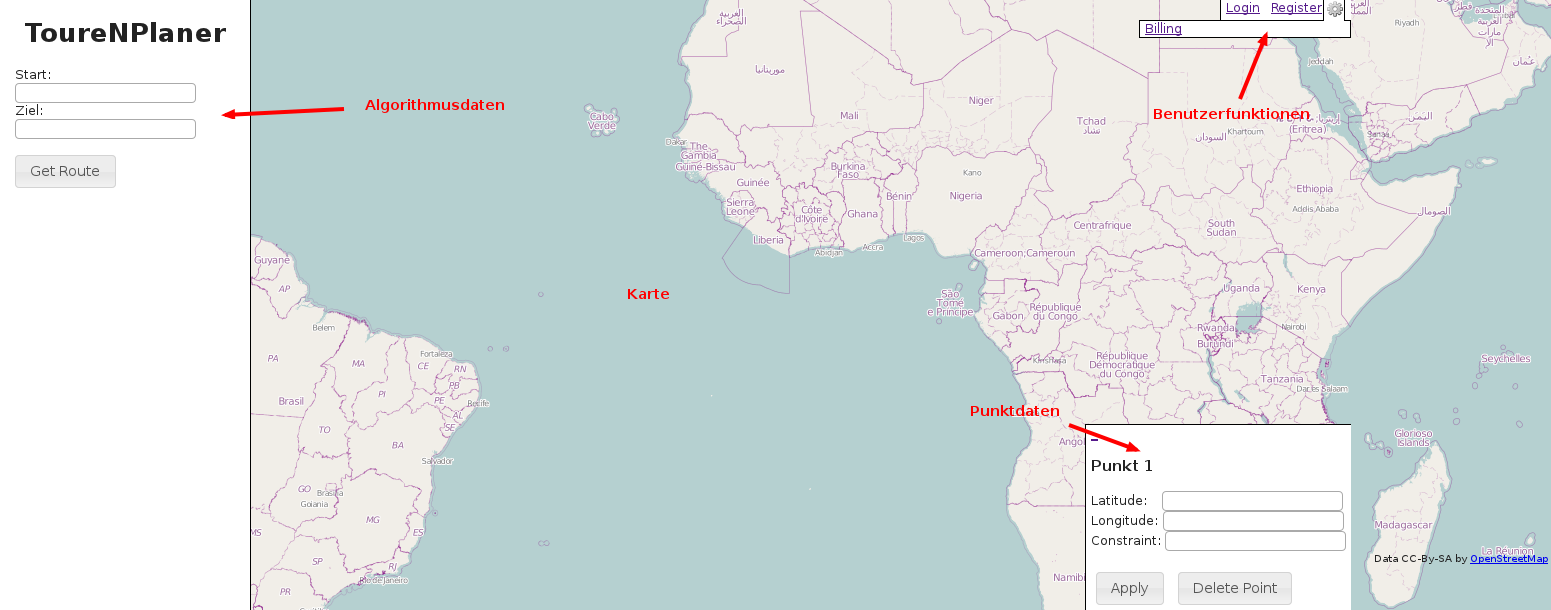
\includegraphics[scale=0.30]{media/web/Index.png} 

\subsubsection{Kartenansicht}
Operationsmöglichkeiten des Benutzers auf der eingeblendeten Kartenansicht.
\begin {itemize}
\item kurzer Linksklick ist nicht definiert
\item kurzer Rechtsklick blendet ein Kontextmenü ein
\item kurzer Linksklick auf einen Marker ermöglicht das Verändern seiner Eigenschaften
\item gedrückter Linksklick ändert den Fokus auf der Karte durch ziehen
\item das Mausrad ermöglicht die Änderung des Zoomfaktors
\end {itemize}
Nachdem die Route berechnet wurde kann das Ergebnis, anhand eines angezeigten Pfades, auf der Karte nachvollzogen werden.

\subsubsection{Die Loginmaske}
In diesem Pop-up kann der Benutzer seine E-mail Adresse und sein Passwort eingeben.
\begin {center}
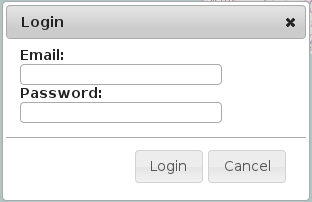
\includegraphics[scale=0.5]{media/web/Login.png}
\end {center}
\subsubsection{Die Registrierungsmaske}
In diesem Pop-up kann der Benutzer die Registrierung durchführen.
\begin {center}
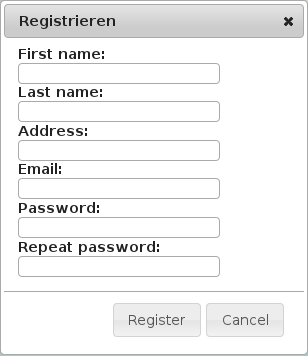
\includegraphics[scale=0.5]{media/web/Register.png}
\end {center}
\subsubsection{Die Billingmaske}
In diesem Pop-up kann sich der Benutzer die Kosten für seine bisherigen Berechnungen anzeigen lassen. Die Maske hinterlegt zusätzlich noch einen Link für jeden Request um diesen nachträglich nocheinmal anzusehen.
\begin {center}
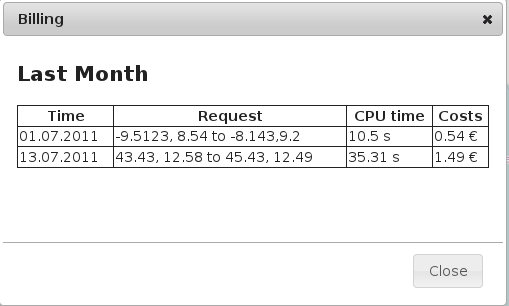
\includegraphics[scale=0.5]{media/web/Billing.png}
\end {center}

\newpage
\subsection{Androidclient}

\subsubsection{Überblick}
Die Benutzeroberfläche des Androidclients ermöglicht folgende Funktionen
\begin{itemize}
\item Auswahl eines Servers
\item Anmeldung mit Benutzernamen und Kennwort
\item Auswahl des gewünschten Algorithmus
\item Auswahl der Billing-Anzeige 
\item Kartenansicht
\item Anlegen eines Markers auf der Karte
\item Zuweisung der Markereigenschaften
\item Zuweisung der Start/Zielpunkte
\item Berechnung der Route
\item Anzeigen der Routen auf der Kartenasicht
\end{itemize}

\subsubsection{Darstellung des Androidclients}
Es folgen nun Layouts aller 'Activities', die als Vorlage zur genauen Realisierung dienen.

\subsubsection{Auswahl des Servers}
Hier kann der Benutzer einen gewünschten Server auswählen. Es wird eine Eingabemaske bereitgestellt um expliziet eine URL einzugeben.
\begin {center}
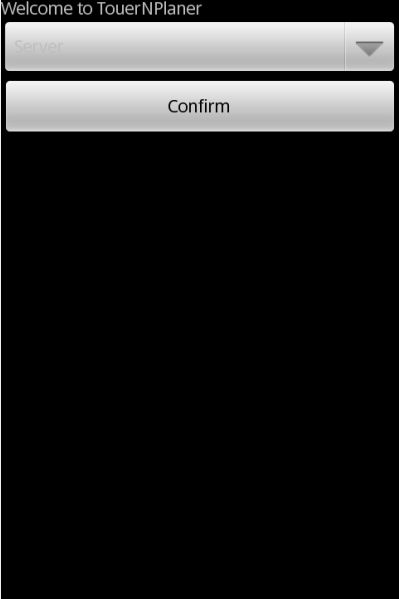
\includegraphics[scale=0.40]{media/android/server.jpg}
\end {center}

\subsection{Anmeldeinformationen}
Hier kann der sich der Benutzer mit seiner E-mail Adresse und Passwort auf dem Server anmelden.
\begin {center}
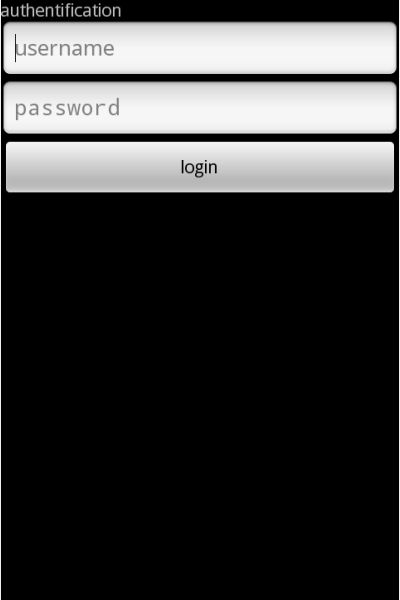
\includegraphics[scale=0.35]{media/android/login.jpg}
\end {center}

\subsection{Algorithmus auswählen}
Hier kann der Benutzer einen Algorithmus auswählen.
\begin {center}
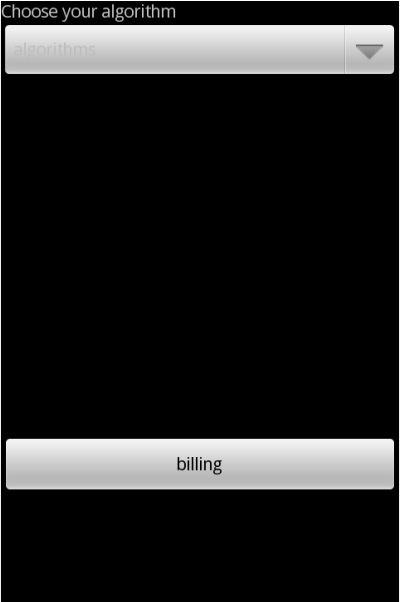
\includegraphics[scale=0.47]{media/android/algorithms.jpg}
\end {center}

\newpage
\subsection{Kartenansicht}
Hier kann der Benutzer, auf der eingeblendeten Kartenansicht, folgende Operationen durchführen:
\begin {itemize}
\item kurzes Drücken ist nicht definiert
\item langes Drücken erstellt einen Marker an dieser Position
\item Drücken auf einen Marker ermöglicht das Verändern seiner Eigenschaften
\item Ziehen auf der Karte ändert den Fokus der Kartenansicht
\item Drücken auf einen der Zoom-Schaltflächen ermöglicht die Änderung des Zoomfaktors
\end {itemize}
Nachdem die Route berechnet wurde kann das Ergebnis, anhand eines angezeigten Pfades, auf der Karte nachvollzogen werden.

\begin {center}
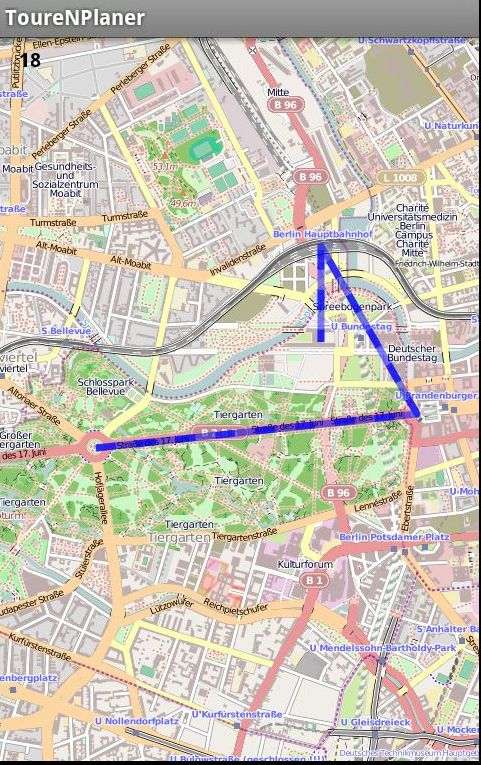
\includegraphics[scale=0.4]{media/android/map.jpg}
\end {center}
\newpage



\clearpage
\section{Anwendungsfälle (Use-Cases)}
\begin{figure}[H]
  \centering
  %TODO
  %\includegraphics[width=\linewidth]{usecases.png}
  \caption{Usecase-Diagramm}
\end{figure}

%\usecase{Name}{Akteur}{Ziel}{Vorbedingung}{Nachbedingung}{Nachbedingung im Sonderfall}{Normalablauf}{Sonderfall}
\subsection*{Benutzeroberflächenfunktionen}
\usecase{Algorithmus auswählen}{Benutzer, Server}{Algorithmus auswählen}{Der Benutzer ist am Server angemeldet}{Der Benutzer hat einen Algorithmus ausgewählt}{Der Benutzer bekommt eine Fehlermeldung}{1. Der Benutzer wählt seinen Algorithmus \newline 2. Benutzer bestätigt seine Eingabe}{Die Verbindung zum Server wurde unterbrochen}

\usecase{Marker hinzufügen}{Benutzer}{Einen Marker auf der Karten hinzufügen}{Die Karte wird angezeigt}{Ein Marker wurde an die gewünschte Stelle plaziert}{Der Marker konnte nicht angelegt werden}{1. Der Benutzer wählt einen gewünschten Punkt auf der Karte \newline 2. Der Benutzer erstellt dort einen Marker}{es besteht bereits ein Marker an dieser Position}

\usecase{Marker editieren}{Benutzer}{Einen vorhandenen Marker editieren}{Ein Marker muss existieren}{Der Marker wurde editiert}{Der Marker wurde auf seine vorherigen Werte zurückgesetzt}{1. Der Benutzer wählt einen Marker aus \newline 2. Der Benutzer ändert die gewünschten Werte des Markers \newline 3. Der Benutzer bestätigt seine Eingaben}{ungültige Eingaben}

\usecase{Marker löschen}{Benutzer}{Einen vorhandenen Marker löschen}{Ein Marker muss vorhanden sein}{Der Marker wurde gelöscht}{keine}{1. Der Benutzer wählt einen Marker aus \newline 2. Der Benutzer bestätigt das Löschen}{keine}

\usecase{Start/Zielpunkt setzen}{Benutzer}{Einen Marker als Ziel/Startpunkt setzen}{Ein Marker muss vorhanden sein}{Ein Marker ist Start/Zielpunkt}{keine}{1. Der Benutzer wählt einen Marker aus \newline 2. Der Benutzer setzt ihn als Start/Zielpunkt}{keine}

\usecase{Route berechnen}{Benutzer, Server}{Eine Route berechnen}{Es müssen Marker auf der Karte plaziert worden sein}{Eine Route wurde berechnet}{Es wird eine Fehlermeldung ausgegeben}{1. Der Benutzer bestätigt seine Eingaben \newline 2. Der Benutzer berechnet seine Route}{Benötigte Angaben für die Berechnung fehlen}

\subsection*{Administrationsfunktionen}
\usecase{Benutzer anlegen}
{Administrator}{Der Administrator will ein Benutzerkonto anlegen.}{Der Administrator ist als solcher eingeloggt.}{Das Konto wurde erfolgreich im System angelegt.}{Der Administrator sieht eine Fehlermeldung.}{
\begin{enumerate}
\item Der Administrator navigiert zum Formular zum Anlegen eines Nutzers.
\item Der Administrator gibt die Daten ein.
\item Der Administrator bestätigt die Angaben.
\end{enumerate}
}{Es gab einen Fehler beim Erstellen des Kontos.}

\usecase{Benutzer bearbeiten}
{Administrator}{Der Administrator will die Daten eines Benutzers bearbeiten.}{Der Administrator ist als solcher eingeloggt.}{Die Daten des Benutzers sind geändert.}{Der Administrator sieht eine Fehlermeldung.}{
\begin{enumerate}
\item Der Administrator wählt einen Benutzer aus.
\item Der Administrator ändert die Daten.
\item Der Administrator bestätigt die Angaben.
\end{enumerate}
}{Es gibt einen Fehler.}

\usecase{Benutzer löschen}
{Administrator}{Der Administrator will einen Benutzer löschen.}{Der Administrator ist als solcher eingeloggt.}{Die Daten des Benutzers und seine alten Abfragen sind gelöscht.}{Der Administrator sieht eine Fehlermeldung.}{
\begin{enumerate}
\item Der Administrator wählt einen Benutzer aus.
\item Der Administrator bestätigt das Löschen.
\end{enumerate}
}{Es gibt einen Fehler.}

\usecase{Benutzer auflisten}
{Administrator}{Der Administrator will eine Lister aller Benutzer sehen.}{Der Administrator ist als solcher eingeloggt.}{Der Administrator kann die Benutzer auswählen.}{Der Administrator sieht eine Fehlermeldung.}{
\begin{enumerate}
\item Der Administrator navigiert zur Benutzerliste.
\end{enumerate}
}{Es gibt einen Fehler.}

\usecase{Benutzer anzeigen}
{Administrator}{Der Administrator will die Daten eines Benutzer sehen.}{Der Administrator ist als solcher eingeloggt.}{Der Administrator sieht die Daten eines Benutzers.}{Der Administrator sieht eine Fehlermeldung.}{
\begin{enumerate}
\item Der Administrator navigiert zur Benutzerliste.
\item Der Administrator wählt einen Benutzer aus.
\end{enumerate}
}{Es gibt einen Fehler.}

\usecase{Abfragen auflisten}
{Administrator}{Der Administrator will eine Liste aller Abfragen sehen.}{Der Administrator ist als solcher eingeloggt.}{Der Administrator sieht alle Abfragen.}{Der Administrator sieht eine Fehlermeldung.}{
\begin{enumerate}
\item Der Administrator navigiert zur Liste aller Abfragen.
\end{enumerate}
}{Es gibt einen Fehler.}

\subsection*{Benutzerverwaltungsfunktionen}
\usecase{Benutzer registrieren}
{Benutzer}{Der Benutzer will sich ein Benutzerkonto anlegen.}{Keine}{Das Konto wurde erfolgreich im System angelegt.}{Der Benutzer sieht eine Fehlermeldung.}{
\begin{enumerate}
\item Der Benutzer navigiert zum Registrierungsformular.
\item Der Benutzer gibt seine Daten ein.
\item Der Benutzer bestätigt seine Angaben.
\end{enumerate}
}{Es gab einen Fehler beim Erstellen des Kontos.}

\usecase{Anmelden}
{Benutzer}{Der Benutzer will sich am System anmelden.}{Keine}{Der Benutzer ist am System angemeldet.}{Der Benutzer sieht eine Fehlermeldung.}{
\begin{enumerate}
\item (optional) Der Benutzer wählt den Server aus.
\item Der Benutzer gibt seine Anmeldedaten ein.
\item Der Benutzer bestätigt seine Angaben.
\end{enumerate}
}{Die Anmeldedaten sind falsch.}

\usecase{Benutzerdaten anzeigen}
{Benutzer}{Der Benutzer will seine Daten einsehen.}{Der Benutzer hat sich eingeloggt.}{Der Benutzer sieht seine Daten.}{Der Benutzer sieht eine Fehlermeldung.}{
\begin{enumerate}
\item Der Benutzer navigiert zur Benutzerdatenansicht.
\item Der Benutzer sieht seine Daten.
\end{enumerate}
}{Es gibt einen Fehler.}

\usecase{Benutzerdaten bearbeiten}
{Benutzer}{Der Benutzer will seine Daten bearbeiten.}{Der Benutzer hat sich eingeloggt.}{Die Daten des Benutzers sind geändert.}{Der Benutzer sieht eine Fehlermeldung.}{
\begin{enumerate}
\item Der Benutzer navigiert zur Benutzerdatenansicht.
\item Der Benutzer ändert seine Daten.
\item Der Benutzer bestätigt seine Angaben.
\end{enumerate}
}{Es gibt einen Fehler.}

\usecase{Abrechnung anzeigen}
{Benutzer}{Der Benutzer will seine Abrechnung sehen.}{Der Benutzer hat sich eingeloggt.}{Der Benutzer sieht seine Abrechnung.}{Der Benutzer sieht eine Fehlermeldung.}{
\begin{enumerate}
\item Der Benutzer navigiert zur Abrechnungsansicht.
\item Der Benutzer sieht seine Abrechnung.
\end{enumerate}
}{Es gibt einen Fehler.}

\usecase{Abfrage anzeigen}
{Benutzer}{Der Benutzer will eine alte Route sehen.}{Der Benutzer hat sich eingeloggt.}{Der Benutzer sieht seine alte Route.}{Der Benutzer sieht eine Fehlermeldung.}{
\begin{enumerate}
\item Der Benutzer navigiert zur Abrechnungsansicht.
\item Der Benutzer wählt eine alte Abfrage aus.
\item Der Benutzer sieht seine alte Abfrage.
\end{enumerate}
}{Es gibt einen Fehler.}

\clearpage
\appendix
\section{Anhang}

\subsection{Begriffslexikon}

%\begriff{Begriff}{Bedeutung}{Abgrenzung}{Gültigkeit}{Bezeichnung}{Unklarheiten}{Querverweise}

\clearpage
\subsection{Versionshistorie}

	\subsubsection*{Version 0.1 (03.08.2011)}
	\begin{itemize}
		\item Erste veröffentlichte Version
	\end{itemize}

	\subsubsection*{Version 0.2 (09.08.2011)}
	\begin{itemize}
		\item Nichtfunktionale Anforderungen hinzugefügt
	\end{itemize}

\end{document}
